\documentclass{article}
\usepackage{tikz}
\usetikzlibrary{arrows}
\usepackage[english]{babel}
\usepackage[utf8]{inputenc}

\usepackage{fancyhdr}
\usepackage{graphicx}
\usepackage{amsmath}
\usepackage[margin=1in]{geometry}

\addtolength{\topmargin}{.2in}
\graphicspath{{./queue_lengths/}}
 
\pagestyle{fancy}
\fancyhf{}
\rhead{Austin Bursey , Aaron Exley\\ Tim McGill, Joseph Myc}
\lhead{CP468 Term Project\\December 2nd  2019}
\rfoot{Page \thepage}
\begin{document}

\begin{titlepage}
  \pagestyle{fancy}
  \thispagestyle{fancy}
   \begin{center}
       \vspace*{1cm}
 
      \Huge
       \textbf{Term Project}
 
       \vspace{0.5cm}
       \Large
        CP468 \\ December 2nd 2019
 
       \vspace{1.5cm}
 
       \textbf{Austin Bursey , Aaron Exley, Tim McGill, Joseph Myc}
 
       \vfill

       \vspace{0.8cm}
 
   \end{center}
\end{titlepage}
\setcounter{page}{2}

\section{How to install/compile/execute our code}
To install the app simply download the .zip file and extract the files wherever you would like to keep the files.
\\
Our code is written in python so no pre-compilation required.\\
\\
We are using some external libraries that need to be installed.  To install these libraries use the following command. The libraries include numpy for faster and easier array calculations and matplotlib to plot graphs\\
\begin{center}
pip install -r requirements.txt
\end{center}
The code can be executed in multiple different ways from command prompt with different arguments:\\

--n [n] for specifying n-queens, 8 otherwise.\\
\\
--file [file] file as input for the initial board state, random otherwise.\\
\\
--maxsteps [steps] the amount queens to move until program should quit looking for a solution, 4000 otherwise. \\

Ex:
\\
To run random 8-queens examples: 
\begin{center}
python n-queens.py
\end{center}
To run random n-queens
\begin{center}
python n-queens.py --n 'n-value here'\\
or\\
python n-queens.py 'n-value'
\end{center}
To run a specific n-queens
\begin{center}
python n-queens.py --file 'file name here'
\end{center}
The format for the input file are as follows; a single digit per line representing the row for the queen. The queens are then filled in from descending order of the text file into the furthest left column of the board all the way to the furthest right in order. 

\section{Design and Implementation choices}
 We used structures like numpy arrays and dictionaries to improve performance. We also created two classes One called Queen which contains two variables; row and col for the row and column value respectively. And Puzzle which contains an array of type Queen which contains all the queens on the belonging to the current board state named 'queens' an array of type queens which contains all the queens currently attacking another queen and a count of all attacking pairs of queens.

\begin{verbatim}



$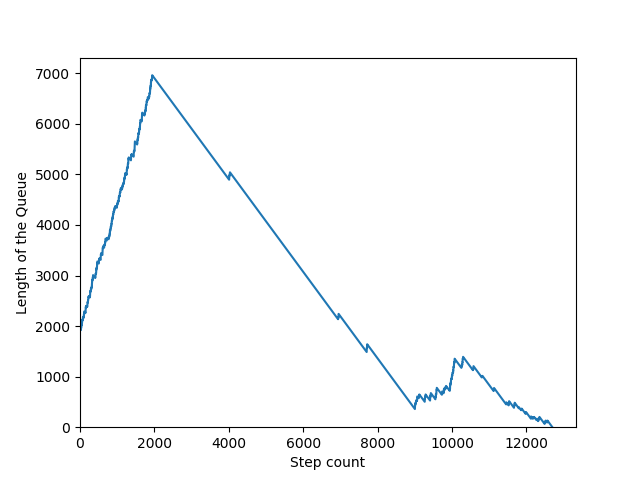
\includegraphics[scale=0.6]{Sudoku-Queue-length-plot-29}$


\end{verbatim}



\end{document}